%!TEX root = ../thesis.tex
\begin{savequote}[75mm]
This Court has long understood that it has a special responsibility to remedy violations of constitutional rights resulting from politicians' districting  decisions...Part of the Court's role in that system is  to  defend its foundations. None is more important than free and fair elections.
\qauthor{Supreme Court Justice Elena Kagan}
\end{savequote}

\chapter{Background and Literature Review}
\label{chap:background}

\section{Racial Gerrymandering and the Courts}

\newthought{Gerrymandering} is the process of manipulating the boundaries of electoral districts to establish an unfair political advantage for some group of people. Racial gerrymandering has been affirmed by the court as a direct violation of constitutional rights, with the Voting Rights Act (VRA) used to further bolster those rights. A racial gerrymander constitutes a ``systemic and infrastructural facet of the practical application of the right to vote,"\cite{greiner} and plaintiffs often invoke the VRA to force officials to redistrict.

Racially polarized voting, defined as different racial groups voting for different candidates in an election, has been central to redistricting law since the 1982 amendments to section 2 of the Voting Rights Act.\cite{greiner} Two kinds of evidence, now known colloquially as the Gingles Test, after the 1986 \textit{Thornburg v. Gingles}\cite{thornburg} case, further codified that in order to prove a violation of the Voting Rights Act one needed to show that:

\begin{enumerate}
 \item the racial or language minority group is sufficiently numerous and compact to form a majority in a single-member district
 \item that group is politically cohesive
 \item and the majority votes sufficiently as a bloc to enable it to defeat the minority’s preferred candidate
\end{enumerate}

The final two requirements require showing racially polarized voting. ``Political cohesion" is often interpreted as racial groups voting for one candidate, and that racial voting information is necessary to determine if racial minority group's candidates are often defeated by the majority racial group's candidates.

This means, practically, that in order to win a lawsuit plaintiffs must prove that voters in districts vote along racial lines. While not every instance of racially polarized voting occurs because of a gerrymandered electoral map, proof of racially polarized voting is often the first step in successfully litigating a racial gerrymandering case as a violation of the VRA.

\subsection{Estimating Racially Polarized Voting}

\newthought{Although} racially polarized voting is critically important to racial gerrymandering litigation, it is quite difficult to prove. The \textit{secret ballot}, an essential part of the United States' democracy, ensures that one's vote is anonymous. Hence, any data collection around voting patterns that separates along any axis of identity, is impossible, and all information about those voting patterns must be inferred.

The \textit{Gingles} decision noted that two techniques were ``standard in the literature for the analysis of racially polarized voting"\cite{thornburg}: bivariate ecological regression and homogeneous precincts.

Dozens of court cases, from the 1980s to now, have relied on either of the above methods for litigating racial gerrymandering cases.\cite{greiner} However, some appellate courts and judges have been hostile to them. In \textit{Lewis v. Alamance County (1996)},\cite{Lewis_Alamance} the court said that the critical assumption of regression ``runs counter to common sense." In \textit{Holder v. Hall (1994)},\cite{Holder_Hall} said that ``bivariate regression analysis...does not directly control for...factors [other than race]."

These criticisms were often ignored by peer and other courts because they did not posit new ways of deciding cases without using regression. Chief Justice Roberts chimed into the debate as well, saying ``At trials, assumptions and assertions give way to facts. In voting rights cases, that is typically done through regression analyses of past voting records."\cite{LULAC}

However, the problem has gotten increasingly more complex. Jim Greiner, Professor of Law at Harvard Law School, stated in his paper \textit{Ecological Inference in Voting Rights Act Disputes: Where Are We Now, and Where Do We Want To Be?}\cite{greiner}

\begin{quote}
 According to some scholars, the patterns themselves have shifted in that a certain percentage of white citizens in some jurisdictions [like Chicago] have become willing to vote for minority-preferred candidates. This shift suggests that the days in which ``documenting racially polarized voting is generally...just beating the obvious" may be gone. Racial bloc voting, often a hotly contested issue in an ``ordinary" redistricting dispute, may now become even more so, and as a result, using the best methodology is more critical.\cite{greiner}
\end{quote}

Greiner's statement is a good introduction to the future of redistricting. He notes not only that the electorate's voting patterns are becoming more complex, but also that to ensure that the courts are equipped with the correct tools to tackle the complexity, the methodologies supplied by and to expert witnesses must be continually improved.

The ecological regression and homogeneous precincts methods had several disadvantages. Ecological regression regularly produces impossible estimates of support, like that $-400\%$ of Hispanic voters in a district supported a candidate. The analysis of homogeneous precincts depends on the assumption that white people living in an all-white precinct vote similarly to white people living in a more racially-diverse precinct, which has been shown empirically, and can be thought intuitively, to be false.\cite{greiner} In addition, neither method generalizes well past $2$ racial groups and $2$ candidates in an election.

The dominant racial bifurcation in both legal and lay discourse is that between Black and white citizens. Thus, much of the litigation of racial gerrymandering and VRA cases, along with the methods used, have focused on these two groups. However, many contemporary cases explore the more complex racial dynamics that exist in our more, and increasingly, diverse electorate.

Take, for example, a recent case that used ecological regression: \textit{League of United Latin American Citizens v. Perry, 126 S. Ct. 2594 (2006)} (LULAC). In this case, Latinx plaintiffs, a mixture of private citizens and representatives of the Mexican American Legal Defense and Educational Fund, argued that Texas' congressional districts were racially gerrymandered to negatively affect Latinx citizens in Texas. With the help of a dubiously-adjusted ecological regression model (to be used for a larger combination of racial groups), the court decided to throw out District 23 within a new plan proposed in 2003, ordering a remedial redistricting.\cite{LULAC} The court also stated that it need not rule that District 25 was a racial gerrymander, given that the remedial changes to District 23 would necessarily affect District 25.

Although not verbally verified by the court, District 25 is widely believed to have been drawn to pack Latinx voters into a district and dilute their voting power, so the redrawing of it and District 23 was a win for that section of the electorate. The change had incredibly practical, and almost immediate, effects. In the year of the remedial redistricting, the affected districts held new primary elections. Henry Bonilla, the Republican representative for the 23rd congressional district, was defeated by Democrat Ciro Rodriguez, a favorite of the Latinx electorate.

Figure \ref{fig:district25} shows the creation of District 25 after the 2003 redistricting in question. Its shape is reminiscent of popular gerrymanders.

\begin{figure*}[ht]\centering
 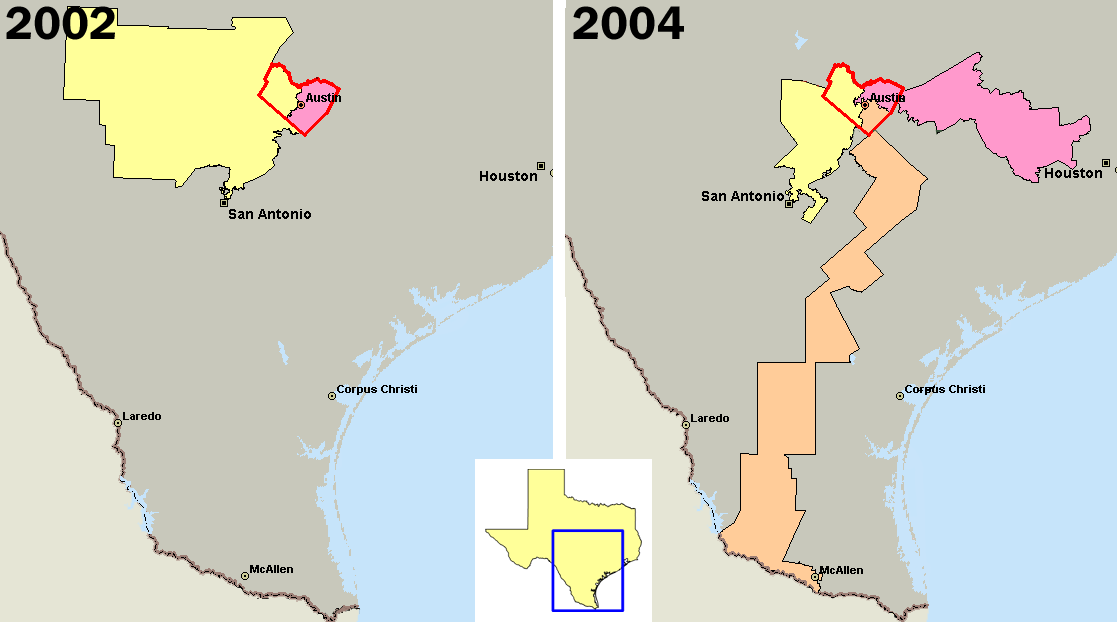
\includegraphics[width=.75\linewidth]{figures/district25.png}
 \caption{The Creation of Texas' 25th Congressional District (orange) in 2003\cite{district25}}
 \label{fig:district25}
\end{figure*}

In that decision, the judges referred to a previous one from 1993, where the court stated:

\begin{quote}
 In countless areas of the law weighty legal conclusions frequently rest on methodologies that would make scientists blush. The use of such blunt instruments in examining complex phenomena and corresponding reliance on inference owes not so much to a lack of technical sophistication among judges, although this is often true, but to an awareness that greater certitude frequently may be purchased only at the expense of other values.\cite{clements}
\end{quote}

Here, the court explicitly acknowledges the disadvantages of the methods used to infer racially polarized voting. These disadvantages, the criticisms lain on ecological regression and homogeneous precincts by some courts, and improvements in theory inspired a burst of energy and innovation in the academy in the late 1990s and early 2000s. At the center of this burst is King's EI.


\section{Ecological Inference}

\newthought{Ecological inference} (EI) is the process of using aggregate (or, ecological) data to infer discrete individual-level relationships of interests when individual-level data are not available.\cite{king1999} This is distinct from the \textit{ecological regression} discussed above, which is the statistical method of running regressions on aggregates and interpreting those regressions as predictive relations on the level of individual units.\cite{ec_reg}

In a world with two categories, groups $\{1, 2, \dots \}$ and groups $\{A, B, \dots \}$, both methods seek to answer the question ``what percentage of members in group $1$ are also in group $A$?" This is precisely the answer that plaintiffs need in racial gerrymandering cases, where groups $\{1, 2, \dots \}$ are races and groups $\{A, B, \dots \}$ are candidates.

Greiner provides an alternate description of EI that fits well within mathematical models.\cite{greiner} EI can also be understood as the attempt to predict internal cell values of a set of contingency tables, like Table \ref{table:ei_example}, when only the column and row totals (the margins of the table) are observed.

\begin{table}
 \centering
 \caption{A $3 \times 3$ Table of Voting By Race, using Counts of Voting Age Population}
 \label{table:ei_example}
 \begin{tabular}{cccc}\toprule
         & Cand. 1       & Cand. 2       & $\sum$        \\\midrule
  Race 1 &      -         &       -        & Race 1 Pop.   \\
  Race 2 &     -          &      -         & Race 2 Pop.   \\
  $\sum$ & Cand. 1 Votes & Cand. 2 Votes & Precinct Pop.
 \end{tabular}
\end{table}

Each precinct has its own table, with an election's vote counts as the column totals and the voting age population, or demographic split of the district, often from the Census, as the row totals. The internal cells, how many people of each racial group that voted for each candidate, are protected by the secret ballot. Those internal cells are exactly the evidence needed in racial gerrymandering litigation, and their values have been inferred by ecological regression and homogeneous precinct analysis in the past.

Theoretically, these tables can be expanded to be as large as necessary: $R \times C$, where $R$ corresponds to the number of rows (demographic groups or races) and $C$ corresponds to the number of columns (candidates). This would be ideal given that the diversification of the electorate has created more politically powerful demographic groups, and that there are frequently more than $2$ candidates in elections, especially in local cases (where many infringements of the VRA are suspected to occur).

Professor Gary King developed and proposed his own method to solve this problem in the late 1990s. It has been used in a few court cases, mainly for the advantage that unlike ecological regression, this method will never produce impossible estimates. It is also understood to be more intuitive than regression, addressing the court's seldom complaint.

\subsection{King's Ecological Inference}

\newthought{Professor King} introduced his method to solve the ecological inference problem in his 1997 book \textit{A Solution to the Ecological Inference Problem: Reconstructing Individual Behavior from Aggregate Data}.\cite{king1997} His method, which he expands upon with several papers from 1997 to the late 2000s, uses Bayesian inference and bounds methods to infer the values of the empty cells in Table \ref{table:ei_example}.

Using Table \ref{table:ei_example} as a reference, Table \ref{table:ei_quantities} describes the quantities that King used to describe this problem.\cite{king1999}

\begin{table*}[ht]
 \centering
 \caption{Quantities in King's EI}
 \label{table:ei_quantities}
 \begin{tabular}{|l|l|}
  \hline
  \multicolumn{1}{|c|}{Quantity} & \multicolumn{1}{|c|}{Description}                           \\
  \hline
  \multicolumn{2}{|c|}{Observed}                                                               \\
  \hline
  $X_i$                          & fraction of population $i$ in race $1$                      \\
  $T_i$                          & fraction of population $i$ who voted for candidate $1$.     \\
  $N_i$                          & size of population $i$                                      \\
  $T'_i$                         & number of people in population $i$ in race $1$              \\
  \hline
  \multicolumn{2}{|c|}{Unobserved}                                                             \\
  \hline
  $b1_i$                         & fraction of members of race $1$ who voted for candidate $A$ \\
  $b2_i$                         & fraction of members of race $2$ who voted for candidate $A$ \\
  \hline
 \end{tabular}
\end{table*}

King's method then uses the observed quantities, and a few parameters, to find the unobserved quantities and answer the ecological inference question. The parameters used are described in Table \ref{table:ei_params}.

\begin{table*}[ht]
 \centering
 \caption{Parameters in King's EI}
 \label{table:ei_params}
 \begin{tabular}{|l|l|}
  \hline
  \multicolumn{1}{|c|}{Parameter} & \multicolumn{1}{|c|}{Description}                                     \\
  \hline
  $c_1, d_1$                     & hyperparameters for the Beta distribution for $b_1$                   \\
  $c_2, d_2$                     & hyperparameters for the Beta distribution for $b_2$.                  \\
  $\theta$                       & the expected fraction of the population of $i$ registered to vote $i$ \\
  $\lambda$                      & the fixed hyperparameter for the distributions of $c_1, c_2, d_1, d_2$ \\
  \hline
 \end{tabular}
\end{table*}

The model is a hierarchical Bayesian inference model that proceeds as follows:

\begin{enumerate}
 \item $c_1, c_2, d_1, d_2 \sim \text{Exponential}(\lambda)$
 \item $b1_i | c_1, d_1 \sim \text{Beta}(c_1, d_1)$
 \item $b2_i | c_2, d_2 \sim \text{Beta}(c_2, d_2)$
 \item $T'_i | b1_i, b2_i, X_i \sim \text{Binomial}(N_i, \theta_i)$
\end{enumerate}

The Python implementation of King's EI is given in Listing \ref{lst:ei_code}. Using the observed quantities, King's method produces a model for the unobserved quantities of interest, which can then be used in litigation as described above.

However, in King's original paper, the bulk of his examples are for $2 \times 2$ tables, and proposed extensions of that method beyond that bound have been dubious.

In King's second iteration of his method and accompanying software, \textit{EI2}, King implements a ``Multiple Imputation Approach" to try to handle $2 \times 3$ tables. In essence, this approach collapses the $2 \times 3$ table into multiple $2 \times 2$ subtables, then applies the original method to each of those subtables.\cite{king2013} Statisticians and scholars, like Jim Greiner, have noted that this method as applied is statistically invalid, as it does not, and cannot, fully adhere to combinatorial rules that the pioneer of multiple imputation, Professor Donald Rubin of Harvard University, notes in his writings.\cite{rubin}

The problems increase if the size of the table increases to $3 \times 3$ or higher. Professor Karen Farree of the University of California, San Diego investigated King's EI applied to tables of that size, and found that the method produced biased estimates and relied on inappropriate modeling assumptions.\cite{ferree}

Hence, although King's method has proved quite useful for some cases of ecological inference, with an increasingly diverse electorate, and complex multi-candidate elections, a method that generalizes well to an $R \times C$ table, using the same data available to previous methods, is necessary.


\section{Discretization}

\newthought{King's method} assumes the quantities of interest, the demographic voting patterns of a district, can be modeled completely with Beta distributions. The hierarchical model allows some freedom to those distributions, generating their parameters from Exponential distributions.

Beta distributions are known to be approximately bimodal if both shape parameters are below $1$. However, Beta distributions can never be \textit{fully} bimodal, which is the expectation for racially polarized voting: that two different groups vote quite differently. Figure \ref{fig:beta_example} is an example of a very, but not fully, bimodal Beta distribution.

\begin{figure}[ht]\centering
 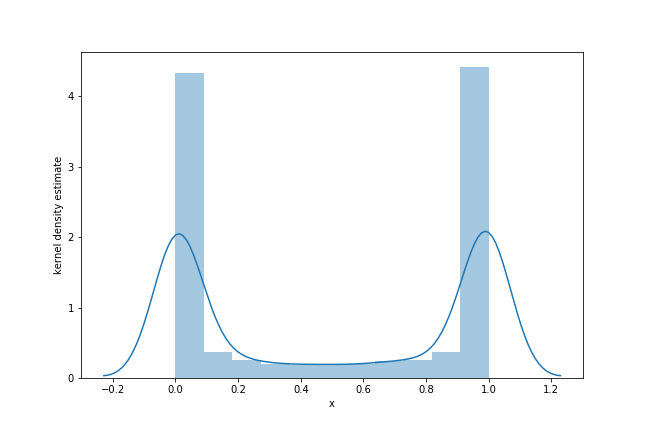
\includegraphics[width=\linewidth]{figures/beta_example.png}
 \caption{Kernel Density Plot of the Beta($0.1$, $0.1$) Distribution}
 \label{fig:beta_example}
\end{figure}

Perhaps more importantly, these distributions can never be multimodal (with more than $2$ modes), which is the case that is necessary for multiple racial groups and candidates. This is where discretization becomes quite useful. Figure \ref{fig:multimodal_example} is an example of a true multimodal distribution over two variables.

A distribution like this could be created easily with Neural Networks, but that architecture requires tens of thousands or millions of data points to be reliable, where a ``data point" would probably be an electoral result. The problem of ecological inference, especially in local elections, is simply too small for those methods.

\begin{figure}[ht]\centering
 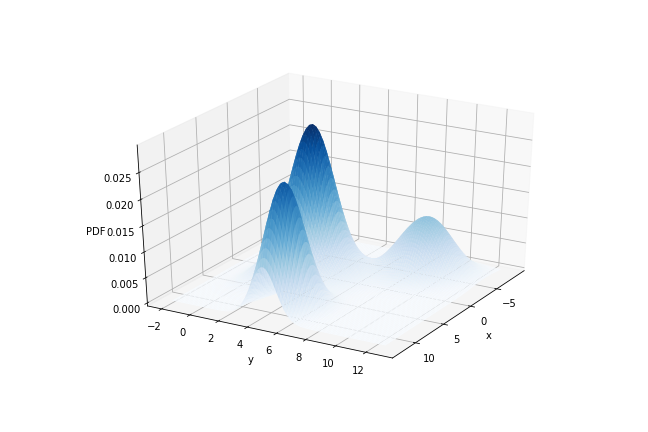
\includegraphics[width=\linewidth]{figures/multimodal_example.png}
 \caption{A Bivariate Multimodal Distribution}
 \label{fig:multimodal_example}
\end{figure}

However, by specifying very little about the space (even less than something like a Beta distribution), then allowing the space to take the shape of the available data, more complex, interesting, and possibly accurate distributions can be found. This is called the \textit{Discrete Voter Model (DVM)}.

For a given candidate, each state of this space is a hypercube (the $n$-dimensional abstraction of a $2$-D square/grid or a $3$-D cube) of values, where each dimension corresponds to a demographic group of interest. Each cell of the hypercube has a probability, where the sum of the probabilities of all cells is $1$. Each cell also uses its position (the values on each axis) in the full hypercube to represent the demographic voting patterns of a given precinct.

For example, in the $2$-dimensional case, for a hypercube with granularity $10$ (each axis goes from $0$ to $10$), let the cell at $(2, 5)$ have an internal probability of $0.4$. This corresponds to there being a $40\%$ chance that this candidate's demographic voting pattern in this precinct is:
\begin{itemize}
  \item $20\%$ of group $1$ votes for them
  \item $50\%$ of group $2$ votes for them
\end{itemize}

Hence, a single hypercube represents the distribution of possible demographic voting patterns in a precinct. Therefore, the distribution of hypercubes represents possibilities for all precincts in a map, and for an election.

The procedure by which the state space of hypercubes takes the shape of the data is Markov chain Monte Carlo.


\subsection{Markov Chain Monte Carlo}

\newthought{Markov chain Monte Carlo (MCMC)} is a class of algorithms that sample from probability distributions that are hard to sample from, typically called \emph{target distributions}.\cite{mcmc_history} With many distributions, like the Normal, Beta, and Exponential mentioned above, obtaining a sample or specifying those distributions is simple and fast. There exist many packages for Python, R, and other programming languages that generate samples instantly with closed form methods.

The target distribution for the Discrete Voter Model, that over the space of hypercubes that could have possibly resulted in the outcome of an election, is not well-specified, and differs not only by election, but also by precinct. Attempting to apply a well-known distribution requires many approximations and assumptions. In lieu of a well-known distribution, the Discrete Voter Model uses discretization and MCMC to find the estimates of the quantities of interest.

All MCMC algorithms are iterative, and the samples converge to the target distribution over time, so the understanding of that target distribution grows with each iteration. All MCMC algorithms construct Markov chains, which means that each sample is generated from, and only depends on, the prior sample in the process, establishing the Markov relationship.\cite{mcmc_methods} At each step, a candidate for the next sample generated according to some transition rules, determined by a \textit{transition kernel}. That candidate is either accepted or rejected based off of some acceptance probability function. More precisely:

Let the chain be represented by ${X_0, X_1, \dots, X_t}$, where $X_i$ is a step in the chain at iteration or time $i$.

Let the target distribution be $\pi(\cdot)$, which has an unnormalized density $\pi_u$.

Let there be some proposal distribution, $Q(\cdot)$, which generates new candidates at every step of the chain. Therefore, as a function $q(x, \cdot)$, it generates $Y_{i + 1}$ as a candidate for $X_{i + 1}$, given $X_i$.

Let there be an acceptance function:

$$\alpha(x, y) = \text{min}\left[1, \frac{\pi_u(y) \cdot q(y, x)}{\pi_u(x) \cdot q(x, y)}\right]$$

The candidate state $Y_{i + 1}$ is accepted with the probability $\alpha(X_i, Y_{i + 1})$. If the state is accepted, $X_{i + 1} \leftarrow Y_{i + 1}$. If not, $X_{i + 1} \leftarrow X_{i}$.

The differences in transition kernels, $Q(x, \cdot)$, and acceptance probability functions, $\alpha(x, y)$, are they key delineators of different types of MCMC algorithms. The Discrete Voter Model uses two types of transition kernels: \textit{Random Walk Metropolis} and \textit{Hamiltonian Monte Carlo}.

\subsection{Random Walk Metropolis}

\newthought{One Markov chain Monte Carlo method} which uses the Random Walk Metropolis transition kernel is the Metropolis-Hastings algorithm. Metropolis-Hastings is one of the simplest MCMC methods, but is still quite reliable and widely used for many applications.

This transition kernel requires that $q(x, y) = q(y - x)$. This is one way to ensure that the chain is reversible and detail balanced, necessary conditions for the chain to converge to the target distribution.\cite{mcmc_rwm}. Examples of such distributions are $Q(x, \cdot) = N(x, \sigma^2)$ and $Q(x, \cdot) = Uniform(x - 1, x + 1)$.

The Discrete Voter Mode's proposal randomly selects two cells in the probability hypercube, and adds a small value, $\epsilon$, to one and subtracts it from the other. This is a reversible chain -- one could get theoretically get back to the probability hypercube that was changed later in the chain -- which is essential for convergence.\cite{mcmc_history}

\subsection{Hamiltonian Monte Carlo}

\newthought{Hamiltonian Monte Carlo} (HMC) differs from Random Walk Metropolis in that its proposal distribution adapts to the current state and its position in the parameter space.\cite{hmc_theory}

HMC uses the gradient of the target distribution's density, and adapts the proposal distribution toward that direction. This helps combat some of the inefficiencies of Random Walk Metropolis, like its tendency to explore parts of the state space where there is very little probability density. Hence, fewer samples have to be created to approximate the target distribution.

The ``Hamiltonian" in ``Hamiltonian Monte Carlo" refers to the inspiration of this kernel: Hamiltonian mechanics, a reformation of Newtonian mechanics that reconsiders the basis of time evolution of a system.\cite{hamiltonian} This kernel generates some \textit{potential function/energy} from the target density, then uses the curvature of that function, some random seed, and the current state to determine the candidate for the next state.\cite{mcmc_hmc}

The primary benefit of HMC to the Discrete Voter Model is that it can theoretically produce a better sample of the target distribution with fewer steps in the algorithm. In addition, HMC has been shown to work well on state spaces with many parameters, like the potentially large probability hypercubes in this model.\cite{mcmc_hmc}

\subsection{Robustness}

\newthought{The Markov chain Central Limit Theorem} guarantees convergence and accurate sampling with the correct specifications.\cite{mcmc_history} Furthermore, for both the kernels above, chains are robust to their assumptions -- they often converge to reliable samples in enough time, even when assumptions (like a perfectly ergodic chain) are broken.

The main disadvantages of using Markov chains for such complex state spaces are that it is difficult to assess convergence, and the methods themselves are computationally expensive. However, given the increasing availability of computing power, including the prevalence of GPU-based computing and the maturity of programming packages like \texttt{Stan}, \texttt{PyMC3}, and \texttt{TensorFlow Probability}, these methods can be more widely applied.
